% Figuras generadas automaticamente por scripts/analyze_medidas.ps1
\begin{figure}[H]
\centering
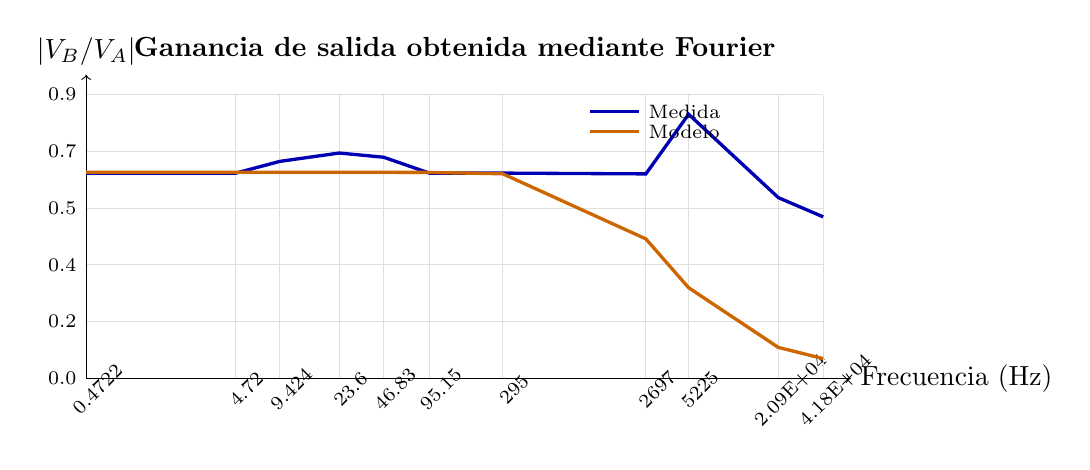
\begin{tikzpicture}[x=0.78cm,y=0.72cm]
\node[font=\bfseries] at (6,5.85) {Ganancia de salida obtenida mediante Fourier};
\draw[gray!25] (0,0) -- (12,0);
\node[left, font=\scriptsize] at (0,0) {0.0};
\draw[gray!25] (0,1) -- (12,1);
\node[left, font=\scriptsize] at (0,1) {0.2};
\draw[gray!25] (0,2) -- (12,2);
\node[left, font=\scriptsize] at (0,2) {0.4};
\draw[gray!25] (0,3) -- (12,3);
\node[left, font=\scriptsize] at (0,3) {0.5};
\draw[gray!25] (0,4) -- (12,4);
\node[left, font=\scriptsize] at (0,4) {0.7};
\draw[gray!25] (0,5) -- (12,5);
\node[left, font=\scriptsize] at (0,5) {0.9};
\draw[gray!25] (0.000,0) -- (0.000,5);
\node[below, font=\scriptsize, rotate=45] at (0.000,0) {0.4722};
\draw[gray!25] (2.425,0) -- (2.425,5);
\node[below, font=\scriptsize, rotate=45] at (2.425,0) {4.72};
\draw[gray!25] (3.154,0) -- (3.154,5);
\node[below, font=\scriptsize, rotate=45] at (3.154,0) {9.424};
\draw[gray!25] (4.121,0) -- (4.121,5);
\node[below, font=\scriptsize, rotate=45] at (4.121,0) {23.6};
\draw[gray!25] (4.843,0) -- (4.843,5);
\node[below, font=\scriptsize, rotate=45] at (4.843,0) {46.83};
\draw[gray!25] (5.589,0) -- (5.589,5);
\node[below, font=\scriptsize, rotate=45] at (5.589,0) {95.15};
\draw[gray!25] (6.782,0) -- (6.782,5);
\node[below, font=\scriptsize, rotate=45] at (6.782,0) {295};
\draw[gray!25] (9.113,0) -- (9.113,5);
\node[below, font=\scriptsize, rotate=45] at (9.113,0) {2697};
\draw[gray!25] (9.809,0) -- (9.809,5);
\node[below, font=\scriptsize, rotate=45] at (9.809,0) {5225};
\draw[gray!25] (11.270,0) -- (11.270,5);
\node[below, font=\scriptsize, rotate=45] at (11.270,0) {2.09E+04};
\draw[gray!25] (12.000,0) -- (12.000,5);
\node[below, font=\scriptsize, rotate=45] at (12.000,0) {4.18E+04};
\draw[->] (0,0) -- (12.45,0) node[right] {Frecuencia (Hz)};
\draw[->] (0,0) -- (0,5.35) node[above] {\(|V_B/V_A|\)};
\draw[very thick, blue!70!black] (0.000,3.614) -- (2.425,3.614) -- (3.154,3.824) -- (4.121,3.971) -- (4.843,3.897) -- (5.589,3.617) -- (6.782,3.617) -- (9.113,3.603) -- (9.809,4.655) -- (11.270,3.184) -- (12.000,2.845);
\draw[very thick, orange!80!black] (0.000,3.632) -- (2.425,3.632) -- (3.154,3.632) -- (4.121,3.632) -- (4.843,3.631) -- (5.589,3.629) -- (6.782,3.605) -- (9.113,2.456) -- (9.809,1.595) -- (11.270,0.542) -- (12.000,0.345);
\draw[very thick, blue!70!black] (8.2,4.7) -- (9.0,4.7); \node[right, font=\scriptsize] at (9.0,4.7) {Medida};
\draw[very thick, orange!80!black] (8.2,4.35) -- (9.0,4.35); \node[right, font=\scriptsize] at (9.0,4.35) {Modelo};
\end{tikzpicture}
\end{figure}
\begin{figure}[H]
\centering
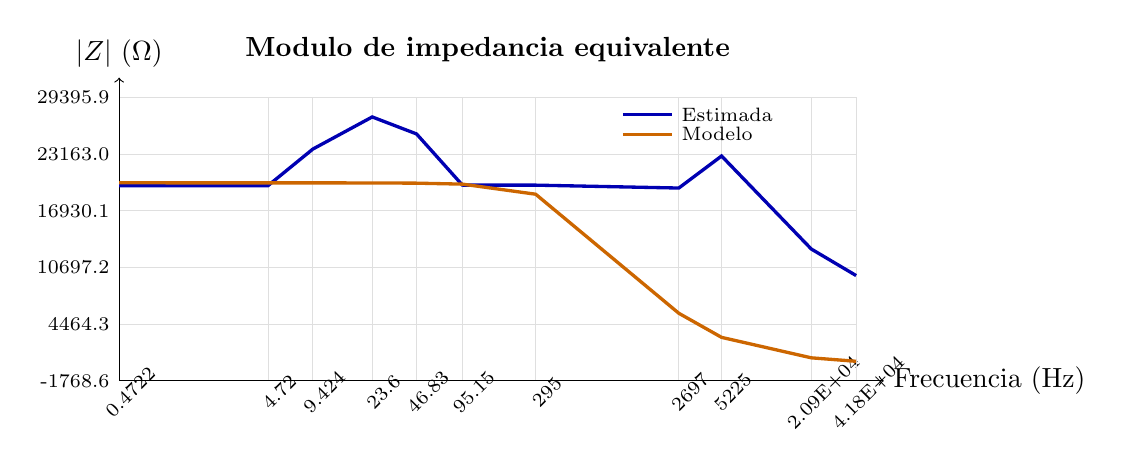
\begin{tikzpicture}[x=0.78cm,y=0.72cm]
\node[font=\bfseries] at (6,5.85) {Modulo de impedancia equivalente};
\draw[gray!25] (0,0) -- (12,0);
\node[left, font=\scriptsize] at (0,0) {-1768.6};
\draw[gray!25] (0,1) -- (12,1);
\node[left, font=\scriptsize] at (0,1) {4464.3};
\draw[gray!25] (0,2) -- (12,2);
\node[left, font=\scriptsize] at (0,2) {10697.2};
\draw[gray!25] (0,3) -- (12,3);
\node[left, font=\scriptsize] at (0,3) {16930.1};
\draw[gray!25] (0,4) -- (12,4);
\node[left, font=\scriptsize] at (0,4) {23163.0};
\draw[gray!25] (0,5) -- (12,5);
\node[left, font=\scriptsize] at (0,5) {29395.9};
\draw[gray!25] (0.000,0) -- (0.000,5);
\node[below, font=\scriptsize, rotate=45] at (0.000,0) {0.4722};
\draw[gray!25] (2.425,0) -- (2.425,5);
\node[below, font=\scriptsize, rotate=45] at (2.425,0) {4.72};
\draw[gray!25] (3.154,0) -- (3.154,5);
\node[below, font=\scriptsize, rotate=45] at (3.154,0) {9.424};
\draw[gray!25] (4.121,0) -- (4.121,5);
\node[below, font=\scriptsize, rotate=45] at (4.121,0) {23.6};
\draw[gray!25] (4.843,0) -- (4.843,5);
\node[below, font=\scriptsize, rotate=45] at (4.843,0) {46.83};
\draw[gray!25] (5.589,0) -- (5.589,5);
\node[below, font=\scriptsize, rotate=45] at (5.589,0) {95.15};
\draw[gray!25] (6.782,0) -- (6.782,5);
\node[below, font=\scriptsize, rotate=45] at (6.782,0) {295};
\draw[gray!25] (9.113,0) -- (9.113,5);
\node[below, font=\scriptsize, rotate=45] at (9.113,0) {2697};
\draw[gray!25] (9.809,0) -- (9.809,5);
\node[below, font=\scriptsize, rotate=45] at (9.809,0) {5225};
\draw[gray!25] (11.270,0) -- (11.270,5);
\node[below, font=\scriptsize, rotate=45] at (11.270,0) {2.09E+04};
\draw[gray!25] (12.000,0) -- (12.000,5);
\node[below, font=\scriptsize, rotate=45] at (12.000,0) {4.18E+04};
\draw[->] (0,0) -- (12.45,0) node[right] {Frecuencia (Hz)};
\draw[->] (0,0) -- (0,5.35) node[above] {\(|Z|~(\Omega)\)};
\draw[very thick, blue!70!black] (0.000,3.443) -- (2.425,3.444) -- (3.154,4.088) -- (4.121,4.655) -- (4.843,4.355) -- (5.589,3.453) -- (6.782,3.452) -- (9.113,3.401) -- (9.809,3.966) -- (11.270,2.325) -- (12.000,1.857);
\draw[very thick, orange!80!black] (0.000,3.493) -- (2.425,3.492) -- (3.154,3.492) -- (4.121,3.491) -- (4.843,3.487) -- (5.589,3.470) -- (6.782,3.292) -- (9.113,1.192) -- (9.809,0.767) -- (11.270,0.406) -- (12.000,0.345);
\draw[very thick, blue!70!black] (8.2,4.7) -- (9.0,4.7); \node[right, font=\scriptsize] at (9.0,4.7) {Estimada};
\draw[very thick, orange!80!black] (8.2,4.35) -- (9.0,4.35); \node[right, font=\scriptsize] at (9.0,4.35) {Modelo};
\end{tikzpicture}
\end{figure}
\begin{figure}[H]
\centering
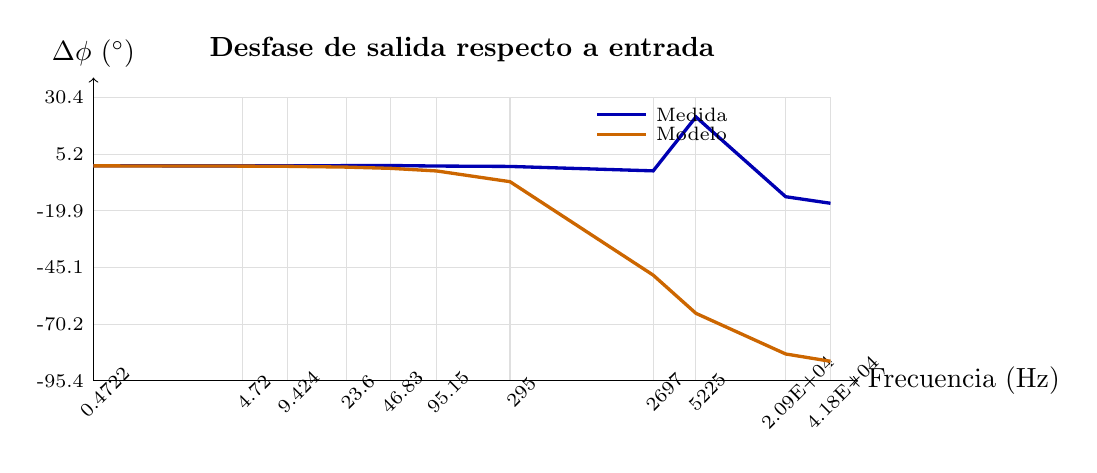
\begin{tikzpicture}[x=0.78cm,y=0.72cm]
\node[font=\bfseries] at (6,5.85) {Desfase de salida respecto a entrada};
\draw[gray!25] (0,0) -- (12,0);
\node[left, font=\scriptsize] at (0,0) {-95.4};
\draw[gray!25] (0,1) -- (12,1);
\node[left, font=\scriptsize] at (0,1) {-70.2};
\draw[gray!25] (0,2) -- (12,2);
\node[left, font=\scriptsize] at (0,2) {-45.1};
\draw[gray!25] (0,3) -- (12,3);
\node[left, font=\scriptsize] at (0,3) {-19.9};
\draw[gray!25] (0,4) -- (12,4);
\node[left, font=\scriptsize] at (0,4) {5.2};
\draw[gray!25] (0,5) -- (12,5);
\node[left, font=\scriptsize] at (0,5) {30.4};
\draw[gray!25] (0.000,0) -- (0.000,5);
\node[below, font=\scriptsize, rotate=45] at (0.000,0) {0.4722};
\draw[gray!25] (2.425,0) -- (2.425,5);
\node[below, font=\scriptsize, rotate=45] at (2.425,0) {4.72};
\draw[gray!25] (3.154,0) -- (3.154,5);
\node[below, font=\scriptsize, rotate=45] at (3.154,0) {9.424};
\draw[gray!25] (4.121,0) -- (4.121,5);
\node[below, font=\scriptsize, rotate=45] at (4.121,0) {23.6};
\draw[gray!25] (4.843,0) -- (4.843,5);
\node[below, font=\scriptsize, rotate=45] at (4.843,0) {46.83};
\draw[gray!25] (5.589,0) -- (5.589,5);
\node[below, font=\scriptsize, rotate=45] at (5.589,0) {95.15};
\draw[gray!25] (6.782,0) -- (6.782,5);
\node[below, font=\scriptsize, rotate=45] at (6.782,0) {295};
\draw[gray!25] (9.113,0) -- (9.113,5);
\node[below, font=\scriptsize, rotate=45] at (9.113,0) {2697};
\draw[gray!25] (9.809,0) -- (9.809,5);
\node[below, font=\scriptsize, rotate=45] at (9.809,0) {5225};
\draw[gray!25] (11.270,0) -- (11.270,5);
\node[below, font=\scriptsize, rotate=45] at (11.270,0) {2.09E+04};
\draw[gray!25] (12.000,0) -- (12.000,5);
\node[below, font=\scriptsize, rotate=45] at (12.000,0) {4.18E+04};
\draw[->] (0,0) -- (12.45,0) node[right] {Frecuencia (Hz)};
\draw[->] (0,0) -- (0,5.35) node[above] {\(\Delta\phi~(^{\circ})\)};
\draw[very thick, blue!70!black] (0.000,3.793) -- (2.425,3.792) -- (3.154,3.793) -- (4.121,3.796) -- (4.843,3.798) -- (5.589,3.789) -- (6.782,3.782) -- (9.113,3.704) -- (9.809,4.655) -- (11.270,3.248) -- (12.000,3.132);
\draw[very thick, orange!80!black] (0.000,3.792) -- (2.425,3.788) -- (3.154,3.784) -- (4.121,3.770) -- (4.843,3.748) -- (5.589,3.702) -- (6.782,3.513) -- (9.113,1.865) -- (9.809,1.191) -- (11.270,0.474) -- (12.000,0.345);
\draw[very thick, blue!70!black] (8.2,4.7) -- (9.0,4.7); \node[right, font=\scriptsize] at (9.0,4.7) {Medida};
\draw[very thick, orange!80!black] (8.2,4.35) -- (9.0,4.35); \node[right, font=\scriptsize] at (9.0,4.35) {Modelo};
\end{tikzpicture}
\end{figure}
